\documentclass[../main.tex]{subfiles}

\usepackage{nopageno} %Seitenzahlen auf richtiger Seite 

\usepackage[left=2cm, right=2cm, top=2cm, includehead, includefoot, headheight=17pt]{geometry}

\usepackage[utf8x]{inputenc}
\usepackage[english]{babel}
\usepackage{amsmath,amssymb,amsthm}
\usepackage{framed}
\usepackage{wasysym}
\usepackage[T1]{fontenc} %Silbentrennung 
\usepackage{color} %Farbe
\usepackage{graphicx}
\usepackage{float}%Grafik am gleichen Ort plazieren
%pdf. png. einfach eingliedern
\usepackage{subfigure} %Grafiken nebeneinander
\usepackage{pdfpages}
\usepackage{ulem} 	%\uuline{urgent}    % doppelt unterstreichen
%\uwave{boat}      % unterschlängeln
%\sout{wrong}       % durchstreichen
%\xout{removed}     % ausstreichen mit //////.

\usepackage{tikz}
\usetikzlibrary{trees}
\usetikzlibrary{plotmarks}
\usetikzlibrary{angles,quotes,babel}
\usetikzlibrary{shadings}
\usetikzlibrary{patterns}
\usetikzlibrary{matrix}
\usetikzlibrary{arrows}
\usetikzlibrary{calc}

\usepackage{pgfplots}
\usepackage{pgf-pie}
\pgfplotsset{compat=1.10}
\usepgfplotslibrary{statistics}
\usepgfplotslibrary{fillbetween}

\usepackage{tkz-euclide}
\usepackage{enumerate}
\usepackage{stmaryrd}
\usepackage{tabularx}
\usepackage{wrapfig}
\usepackage{epsdice}
\usepackage{multirow}
\usepackage{rotating}
\usepackage{pdflscape}
\usepackage{fancyhdr}

\pagestyle{fancy} %eigener Seitenstil
\fancyhf{} %alle Kopf- und Fußzeilenfelder bereinigen
\fancyhead[L]{} %Kopfzeile links
\fancyhead[C]{} %zentrierte Kopfzeile
\fancyhead[R]{} %Kopfzeile rechts
\renewcommand{\headrulewidth}{0.4pt} %obere Trennlinie
\fancyfoot[C]{\thepage} %Seitennummer
\renewcommand{\footrulewidth}{0.4pt} %untere Trennlinie

% Number spaces 
\newcommand{\CC}{\ensuremath{\mathbb{C}}}
\newcommand{\RR}{\ensuremath{\mathbb{R}}}
\newcommand{\QQ}{\ensuremath{\mathbb{Q}}}
\newcommand{\ZZ}{\ensuremath{\mathbb{Z}}}
\newcommand{\NN}{\ensuremath{\mathbb{N}}}
\newcommand{\LL}{\ensuremath{\mathbb{L}}}
\newcommand{\DD}{\ensuremath{\mathbb{D}}}
\newcommand{\WW}{\ensuremath{\mathbb{W}}}

%draw chemestry molecules 
\usepackage{chemfig} % https://mirror.ox.ac.uk/sites/ctan.org/macros/generic/chemfig/

\newcommand\vv[1]{%
	\begin{tikzpicture}[baseline=(arg.base)]
		\node[inner xsep=0pt] (arg) {$#1$};
		\draw[line cap=round,line width=0.45,->,shorten >= 0.2pt, shorten <= 0.7pt] (arg.north west) -- (arg.north east);
	\end{tikzpicture}%
} %command will render \vv{x} with an arrow aboth 

\renewcommand{\labelenumi}{\roman{enumi})}

\DeclareMathOperator{\ggT}{ggT}
\DeclareMathOperator{\sign}{sign}

%sections
\theoremstyle{plain}
\newtheorem{Thm}{Theorem}[section]
\newtheorem{Def}[Thm]{Definition}
\newtheorem{Prop}[Thm]{Proposition}

\theoremstyle{definition}
\newtheorem{lemma}[Thm]{Lemma}
\newtheorem{corollary}[Thm]{Corollary}
\newtheorem{claim}[Thm]{Claim}
\newtheorem{Proof}[Thm]{Proof}
\newtheorem{Ex}[Thm]{Example}

\newtheorem{Exercise}{ex}[section] %follow proper enum
\newtheorem{ex}[Exercise]{Exercise}
\newtheorem{Solution}{sol}[section]
\newtheorem{sol}[Solution]{Solution}

\theoremstyle{remark}
\newtheorem{remark}[Thm]{Remark} % follows thm enum

\newtheorem{comment}{Comment}[section] %follow comment enum
\newtheorem{notation}[comment]{Notation}
\newtheorem{reasoning}[comment]{Reasoning}
\newtheorem{Intpr}[comment]{Interpretation}

%some premmade with title (uterwise use \textbf{Title} ...)
\newenvironment{ThmWithTitle}[1]{%
	\begin{Thm}[\textbf{#1}]}{\end{Thm}}
\newenvironment{PropWithTitle}[1]{%
	\begin{Prop}[\textbf{#1}]}{\end{Prop}}
\newenvironment{ExWithTitle}[1]{%
	\begin{Ex}[\textbf{#1}]}{\end{Ex}}
\newenvironment{DefWithTitle}[1]{%
	\begin{Def}[\textbf{#1}]}{\end{Def}}
\newenvironment{RemarkWithTitel}[1]{%
	\begin{remark}[\textbf{#1}]}{\end{remark}}

%format of paragraph 
\renewcommand\paragraph{\@startsection{paragraph}{4}{\z@}%
	{-2.5ex\@plus -1ex \@minus -.25ex}%
	{1.25ex \@plus .25ex}%
	{\normalfont\normalsize\bfseries}}
\makeatother
\setcounter{secnumdepth}{4} % how many sectioning levels to assign numbers to
\setcounter{tocdepth}{4}    % how many sectioning levels to show in ToC

\newcounter{row} 
\renewcommand\therow{\alph{row}} %hier a,b,c etc. def und mit therow abrufbar

\newenvironment{aufz}
{\setcounter{row}{0}%
	\par\noindent\tabularx{\linewidth}[t]
	{\cdot{20}{>{\stepcounter{row}\makebox[1.5em][l]{\therow)\hfill}}X}} %bis max 20 Elemente nebeinander
}
{\endtabularx}


%biblio
\usepackage[]{biblatex}
\addbibresource{referenzenma.bib} 

%glossary
\usepackage{glossaries}
\usepackage{import}


\usepackage{rotating} % Include this package in the preamble

\newglossaryentry{Enzyme}{
	name={Enzyme},
	description={A macromolecular biological catalyst that significantly accelerates chemical reactions, often with high specificity. They can be proteins or catalytically active RNA molecules.
}}

\newglossaryentry{Cofactor}{
	name={Cofactor},
	description={An inorganic chemical component required for enzyme activity. Often metal ions such as Fe\textsuperscript{2+}, Mg\textsuperscript{2+}, or Zn\textsuperscript{2+}.
}}

\newglossaryentry{Coenzyme}{
	name={Coenzyme},
	description={A complex organic or metallorganic molecule required for enzyme function, often derived from vitamins. Acts as a transient carrier of specific functional groups.
}}

\newglossaryentry{Systematic name}{
	name={Systematic name},
	description={A precise name given to an enzyme that indicates the substrates and type of reaction it catalyzes (e.g., ATP:glucose phosphotransferase for hexokinase).
}}

\newglossaryentry{Classification number}{
	name={Classification number},
	description={A four-part code assigned to enzymes based on the type of reaction they catalyze (e.g., 2.7.1.1 for hexokinase).
}}

\newglossaryentry{Activation Energy}{
	name={Activation Energy},
	description={The energy barrier ($$\Delta G^{\ddagger}$$) between the ground state and the transition state that must be overcome for a reaction to proceed.
}}

\newglossaryentry{Transition State Theory}{
	name={Transition State Theory},
	description={A model describing the top of the energy hill in a reaction coordinate where reactants are equally likely to proceed to products or return to reactants. Not to be confused with reaction intermediates.
}}

\newglossaryentry{Transition State}{
	name={Transition State},
	description={The highest-energy configuration along the reaction coordinate. It is the point at which the system is equally likely to proceed toward products or return to reactants. It is not a stable intermediate and is denoted as $\ddagger$.
}}


\newglossaryentry{Reaction Intermediate}{
	name={Reaction Intermediate},
	description={A short-lived, chemically distinct species that occurs during the transformation of reactants to products, such as enzyme-substrate (ES).
}}

\newglossaryentry{K_{eq}}{
	name={$K_{eq}$},
	description={The equilibrium constant of a reaction, given by the ratio $$\frac{[P]}{[S]}$$. Not affected by enzymes.
}}

\newglossaryentry{Delta G}{
	name={$\Delta G$},
	description={The change in free energy during a reaction. $\Delta G°$ refers to standard conditions, and $\Delta G°^{\prime}$ includes biochemical conditions (pH = 7).
}}

\newglossaryentry{Delta G dagger}{
	name={$\Delta$ $G^{\ddagger}$},
	description={The activation free energy, the difference in energy between the ground state and the transition state.
}}

\newglossaryentry{Return Rate}{
	name={Return Rate},
	description={The rate of the reaction based on substrate concentration and a rate constant $$k$$, where $$v = k[S]$$.
}}

\newglossaryentry{Catalytic Power}{
	name={Catalytic Power},
	description={The ability of enzymes to lower the activation energy and provide alternate reaction pathways, enhancing the reaction rate.
}}

\newglossaryentry{Active Site}{
	name={Active Site},
	description={The region of the enzyme where substrate binding and catalysis occur, often through specific amino acid residues.
}}

\newglossaryentry{Transition State Complementarity}{
	name={Transition State Complementarity},
	description={The enzyme binds more tightly to the transition state than to the substrate, thereby lowering the activation energy and enhancing catalysis.
}}

\newglossaryentry{Rate Enhancement}{
	name={Rate Enhancement},
	description={The increase in reaction speed due to the lowering of the activation energy by enzyme catalysis.
}}

\newglossaryentry{Binding}{
	name={Binding},
	description={The specific interaction between enzyme and substrate, often involving multiple weak noncovalent interactions to drive catalysis.
}}

\newglossaryentry{Specificity}{
	name={Specificity},
	description={The enzyme's ability to select exact substrates and catalyze a specific reaction, influenced by binding energy and structural complementarity.

\newglossaryentry{Acid-Base Catalysis}{
	name={Acid-Base Catalysis},
	description={A catalytic mechanism in which amino acid residues act as proton donors or acceptors to stabilize charged intermediates, increasing reaction rates when water alone is insufficient.
}}

#ab hier sollten keine Komma Probleme mehr sein.

\newglossaryentry{Covalent Catalysis}{
	name={Covalent Catalysis},
	description={A mechanism where the enzyme forms a transient covalent bond with the substrate, creating an alternative reaction pathway with lower activation energy. This requires nucleophilic groups on the enzyme.}
}

\newglossaryentry{Metal Ion Catalysis}{
	name={Metal Ion Catalysis},
	description={Catalysis involving metal ions that can stabilize negative charges on reaction intermediates, help substrate orientation, or mediate redox reactions through reversible changes in oxidation state.}
}

\newglossaryentry{Enzyme Kinetics}{
	name={Enzyme Kinetics},
	description={The study of the rate of enzyme-catalyzed reactions and how they change in response to experimental parameters like substrate concentration.}
}

\newglossaryentry{v_0}{
	name={$v_0$},
	description={The initial velocity of an enzyme-catalyzed reaction, measured at the very beginning before product accumulates. At low $[S]$, $v_0$ increases almost linearly with $[S]$.}
}

\newglossaryentry{Enzyme Saturation}{
	name={Enzyme Saturation},
	description={The condition where increasing substrate concentration no longer increases the reaction rate because all active sites are occupied, resulting in a plateau at $v_{max}$.}
}

\newglossaryentry{v_{max}}{
	name={$v_{max}$},
	description={The maximal velocity of an enzyme-catalyzed reaction when all enzyme molecules are saturated with substrate. Defined by $v_{max} = k_{cat}[E]_T$.}
}

\newglossaryentry{Michaelis-Menten}{
	name={Michaelis-Menten},
	description={A kinetic model describing enzyme activity: $v_0 = \frac{v_{max}[S]}{K_m + [S]}$, where $K_m$ is the substrate concentration at half-maximal velocity.}
}

\newglossaryentry{Lineweaver-Burk}{
	name={Lineweaver-Burk},
	description={A double reciprocal plot of enzyme kinetics: $\frac{1}{v_0} = \frac{K_m}{v_{max}} \cdot \frac{1}{[S]} + \frac{1}{v_{max}}$, used to linearize the Michaelis-Menten equation for easier interpretation.}
}

\newglossaryentry{Enzyme Efficiency}{
	name={Enzyme Efficiency},
	description={Measured by the specificity constant $\frac{k_{cat}}{K_m}$, which reflects both substrate binding and catalytic turnover. The theoretical upper limit is $10^8$ to $10^9 \text{ M}^{-1}\text{s}^{-1}$.}
}

\newglossaryentry{Inhibition}{
	name={Inhibition},
	description={The decrease or complete loss of enzyme activity due to the binding of a molecule (an inhibitor) that interferes with catalysis. Inhibition is fundamental to drug action and metabolic regulation.}
}

\newglossaryentry{Reversible Inhibition}{
	name={Reversible Inhibition},
	description={Inhibition where the inhibitor binds non-covalently and can dissociate from the enzyme. Includes competitive, non-competitive, and uncompetitive mechanisms.}
}

\newglossaryentry{Competitive Inhibitor}{
	name={Competitive Inhibitor},
	description={A molecule that competes with the substrate for binding at the active site. It increases $K_m$ but does not affect $v_{max}$.}
}

\newglossaryentry{Non-competitive Inhibitor}{
	name={Non-competitive Inhibitor},
	description={Binds to a site other than the active site and reduces the effective concentration of active enzyme. It decreases $v_{max}$ without changing $K_m$.}
}

\newglossaryentry{Uncompetitive Inhibitor}{
	name={Uncompetitive Inhibitor},
	description={Binds only to the enzyme-substrate complex, preventing product formation. It decreases both $v_{max}$ and $K_m$.}
}

\newglossaryentry{Irreversible Inhibition}{
	name={Irreversible Inhibition},
	description={Inhibition where the inhibitor covalently binds or permanently inactivates the enzyme, preventing further catalytic activity.}
}

\newglossaryentry{Suicide Inhibition}{
	name={Suicide Inhibition},
	description={A special type of irreversible inhibition where the enzyme converts the inhibitor into a reactive intermediate that covalently modifies and inactivates the enzyme.}
}

\newglossaryentry{Transition-State Analogs}{
	name={Transition-State Analogs},
	description={Stable molecules that resemble the transition state of a substrate and bind tightly to the enzyme, acting as potent inhibitors by exploiting transition state complementarity.}
}



\makeglossaries

\begin{document}
	

\section{Enzymes}

\subsection{What is an Enzyme: Overview and Components}

An \gls{Enzyme} is a macromolecular biological catalysts that extraordinarily accelerate chemical reactions ($10^{6}$ fold). Enzymes possess a high degree of specificity. Enzymes are essential to the metabolism by conserving and transforming chemical energy as well as synthesizing biological macromolecules from simple precursors. Approximately 50\% of drugs act by binding to enzymes. 

Enzymes are either composed of either proteins or catalytically active RNA molecules. They can require additional components such as cofactors or helpers a.k.a. coenzymes.

\subsubsection{Cofactors and Coenzymes}

\textbf{\gls{Cofactor}}: A cofactor is a chemical component, often an inorganic ion.
\textbf{\gls{Coenzyme}}: A Coenzyme is a complex organic or metallorganic molecules. Vitamins are precursors of coenzymes.

\begin{figure}[h]
	\centering
	\subfigure[Cofactors]{
		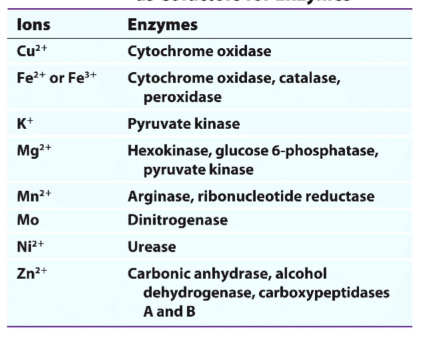
\includegraphics[width=0.45\textwidth]{Cofactors}
	}
	\hfill
	% Second subfigure
	\subfigure[Coenzymes]{
		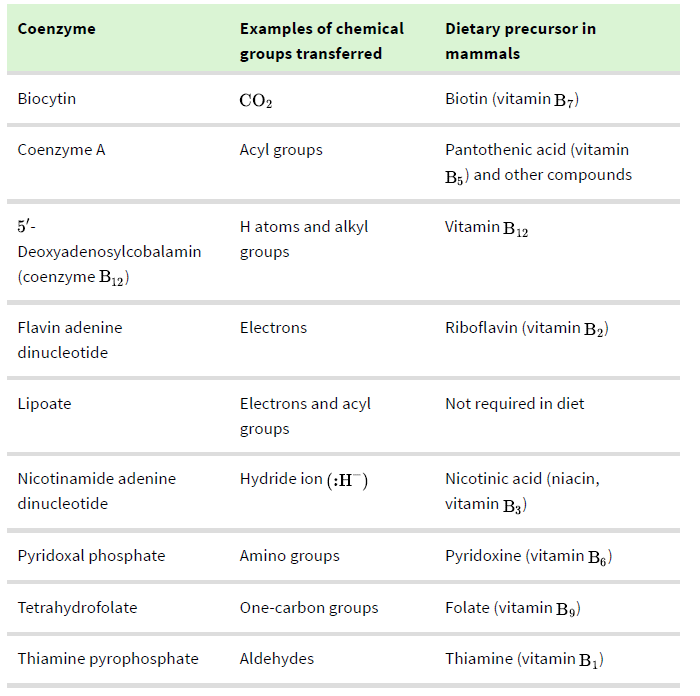
\includegraphics[width=0.5\textwidth]{Coenzymes}
	}
	\caption{Examples of Cofactors and Coenzymes}
\end{figure}

\subsubsection{Enzymes Classification}
Enzymes are named by adding the suffix "-ase" to the name of their substrate or activity. The more formal version is assigning each enzyme a four-part classification number and a systematic name.
\textbf{\gls{Systematic name}}: Includes its precise activity and the substrates it works with (e.g., hexokinase is ATP:glucose phosphotransferase).
\textbf{\gls{Classification number}}: Four number code, using again Hexokinase (2.7.1.1) as an example:
\begin{enumerate}
	\item Class name (2: Transferase)
	\item Subclass name (7: Phosphotransferase)
	\item The acceptor functional group (1: Phosphotransferase with hydroxyl group as acceptor)
	\item The accepting molecule (1: D-Glucose as acceptor molecule)
\end{enumerate} 

\begin{figure}[h]
	\centering
	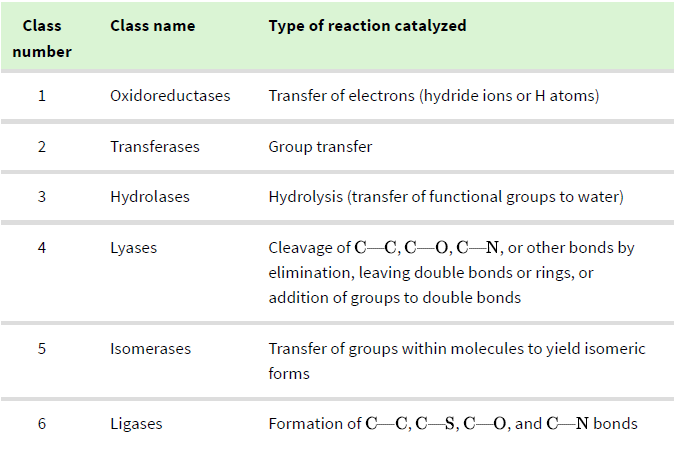
\includegraphics[width=0.45\textwidth]{Enzyme_classification}
	\caption{Examples of Cofactors and Coenzymes}
\end{figure}

\subsection{The Thermodynamics and an Enzymes Role}
\textbf{Enzymes reduce the \gls{Activation Energy} for a given reaction, hence changing the rate of the reaction. They do not influence $K_{eq}$ or $\Delta$G}

\begin{figure}[h]
	\centering
	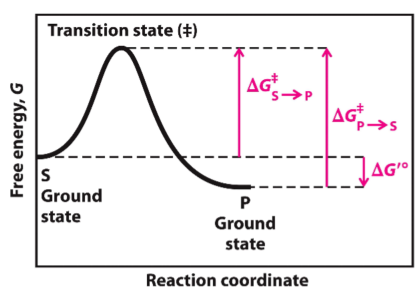
\includegraphics[width=0.45\textwidth]{Reaction_diagram}
	\caption{A reaction diagram}
\end{figure}

\subsubsection{\gls{Transition State Theory}}
When plotting the progress of a reaction the \gls{Transition State} is the very top of the hill. Note, that the \textbf{transition state $\neq$ \gls{Reaction Intermediate}}. It should be understood as the moment in which the reaction is equally likely to progress towards substrate or product.




\subsubsection{\gls{K_{eq}}}
The equilibrium constant $K_{eq}$, or K, is the reaction quotient at chemical equilibrium. K gives is calculated by:
\begin{equation}
	K = \frac{[P]}{[S]}
\end{equation}

\textbf{An enzyme has no effect on K}.

$K'_{eq}$ is the $K_{eq}$ at standard biochemical conditions (298K, pH = 7).


\subsubsection{\gls{Delta G} and \gls{Delta G dagger}}

The activation energy ($\Delta$G$\ddagger$) is the difference between the ground state and the transition state.

$\Delta$G° is the standard free energy under standard conditions (T = 298K, 1atm, 1M of each solute), while $\Delta$G'° is also at pH = 7.
\subsubsection{The Relationship Between \gls{K_{eq}} and \gls{Delta G}}
\begin{equation}
	\Delta G^\circ{}' = -RT \ln K'_{\mathrm{eq}}
\end{equation}

where, \( R = 8.315\, \frac{\mathrm{J}}{\mathrm{mol \cdot K}} \) and \( T = 298\, \mathrm{K} \). \\

Note that large K $\leftrightarrow$ very negative $\Delta$G'°

\begin{figure}[h]
	\centering
	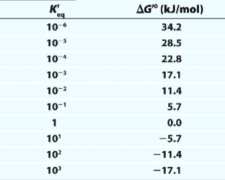
\includegraphics[width=0.45\textwidth]{G_and_K}
	\caption{Some examples showing the relationship between G and K}
\end{figure}

\subsubsection{\gls{Return Rate}}
The rate of a reaction is determined by the concentration of the reactants and the rate constant k.

For a unimolecular reaction we have that
\begin{equation}
	v = k[S]
\end{equation}

in which the reaction only depends on [S] and k has units $s^{-1}$ and the following formula:

\begin{equation}
	k = \frac{k'T}{h} * e^{-\frac{\Delta G \ddagger}{RT}}
\end{equation}

where k' is the Boltzmann constant and h the Plank constant. This means that the lower $\Delta$G$\ddagger$ the faster the reaction goes. Since, enzymes lower $\Delta$G$\ddagger$ it raises k and voila reaction is now speedy Gonzo.

\begin{figure}[h]
	\centering
	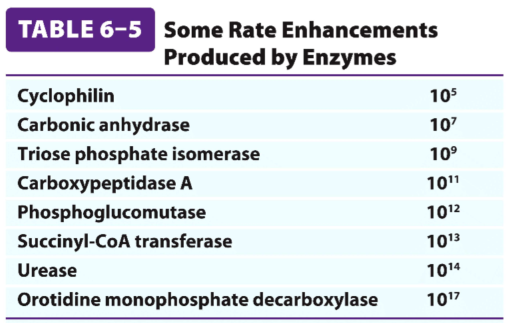
\includegraphics[width=0.45\textwidth]{Enzymes_speedo}
	\caption{Some Rate enhancements Produced by Enzymes}
\end{figure}

\subsection{Enzymes' Role in the Reaction}

To piece it all together an enzyme does the following:
\begin{itemize}
	\item Has no effect on equilibrium related things; it does not influence G or K;
	\item Lowers the energy of $\Delta$G$\ddagger$ and with it the activation energy;
	\item Hence creating a larger k and with that speeding up the rate of the reaction.
\end{itemize}

\begin{figure}[h]
	\centering
	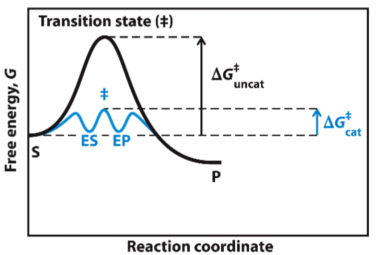
\includegraphics[width=0.45\textwidth]{Enzyme_RD}
	\caption{The Enzyme introduces a couple of new transition states (ES and EP), each of which is more stable than the original transition state}
\end{figure}

This speeding up happens due to three main things:

\subsubsection{\gls{Catalytic Power} and Mechanism}
An enzyme has two ways to make a reaction faster:
\begin{enumerate}
	\item Providing a \textbf{lower-energy reaction path}.
	\item Releasing energy through the \textbf{non-covalent binding} between the substrate and the enzyme. That energy is referred to as \textbf{$\Delta$G$_{B}$}. This energy gain is a major driving force for the reaction to even happen
\end{enumerate}

PSA: Your friendly reminder that the enzyme will remain unchanged when comparing beginning and end of reaction!

\subsubsection{\gls{Active Site}}

The active site is the place of the reaction. This site is lined with amino acids residue, which possess qualities to bind to the substrate and catalyze its transformation. Often times an enzymes will envelop a  substrate separating it from the solution.

This binding is highly specific. This is where the lock and key principal comes into play. However it is slightly misleading as then the transition state would have to be more unfavorable than the  substrate. Hence, it is more precise to see the \textbf{enzyme as very specific to the transition state} (which is till similar to the substrate).

\subsubsection{Example for \gls{Transition State Complementarity} and \gls{Rate Enhancement}}
Using the example of stickase we show the importance of the transition state complementarity, the fault of lock and key, and how that leads to rate enhancement.

No enzyme:
\begin{figure}[h]
	\centering
	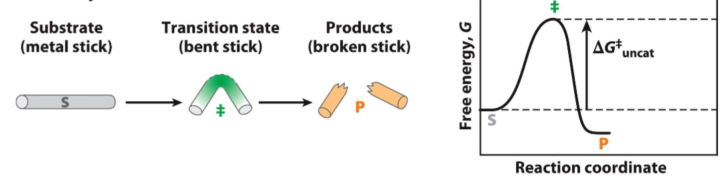
\includegraphics[width=0.45\textwidth]{stick_no}
\end{figure}

Enyzme which is complementary to the substrate:
\begin{figure}[h]
	\centering
	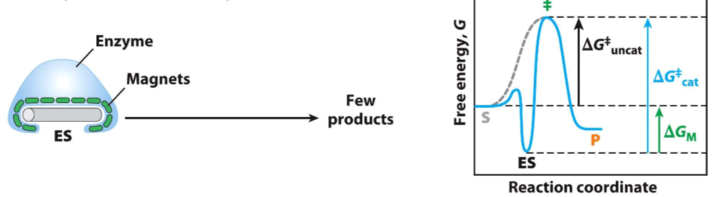
\includegraphics[width=0.45\textwidth]{stick_s}
	\caption{because the enzyme is complementary to the substrate it will stabilize the stick, making the ES state the most stable one and the required $\Delta$G$\ddagger$ larger than without an enzyme.}
\end{figure}

Enzyme which is complementary to the transition state:
\begin{figure}[h]
	\centering
	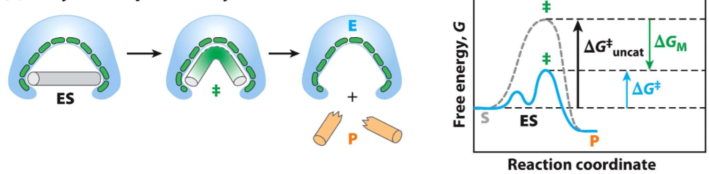
\includegraphics[width=0.45\textwidth]{stick_ts}
	\caption{With the enzyme being complementary to the TS, the ES-state would still be more favorable, but not too favorable. More importantly the $\Delta$G$\ddagger$ would be lowered as the TS is significantly more stable.}
\end{figure}

\subsubsection{\gls{Binding} and \gls{Specificity}}

There are numerous not favorable physical and thermodynamical factors which contribute to $\Delta$G$\ddagger$, which need to be overcome:
\begin{enumerate}
	\item \textbf{freedom through entropy}: The motion of molecules which reduces the possibility of proximity and hence reaction;
	\item \textbf{Solvation of the water shell}
	\item \textbf{Distortion of substrates}
	\item\textbf{ proper alignment} of the catalytic functional groups on the enzyme
\end{enumerate}

All these factors are overcome by the binding energy, which is released once ES enter the transition state. The need for this binding energy further enhances specificity. Here is how exactly the binding energy comes to be and is favorable:

\begin{enumerate}
	\item \textbf{Entropy Reduction}: Through the binding of substrates to the enzyme, the freedom of motion of the substrates is significantly limited. This leads to the probability that they collide to react skyrocketing.
	\item \textbf{Desolvation}: Due to the binding of enzyme and substrate water molecules are are removed. While locally that means a slight decrease in entropy, overall it leads to an increase, making it energetically favorable.
	\item \textbf{Substrate Distortion}: The binding energy we get later on formed through the transition state and enzyme help compensate for any initial distortion, especially electronic redistribution.
	\item \textbf{Catalytic Group alignment}: As the substrate binds to the enzyme, the enzyme undergoes a so called induced fit, meaning it envelops the substrate in such a way that its functional groups can properly catalyze at the right position, as well as put the reaction sites of the substrates in the right position.
\end{enumerate}

All these barriers and conditions to resolve them, make an enzyme very specific in which molecules it can catalyze. Those that work however, it is then able to create a huge rate enhancement.


\subsection{Other Contributions to Enzyme Catalysis}

Intermediates can often be very unstable, making them very unfavorable to get to (high $\Delta$G$\ddagger$). Here are some ways enzymatic complexes overcome this and hence enhance reaction rates:

\begin{enumerate}
	\item \textbf{\gls{Acid-Base Catalysis}}: Some intermediates will be charged, which can lead to great instability. In order to stabilize them protonating/deprotonating can create a much more stable intermediate. Since water is rather weak, it will often be catalyzed with an amino acid residue which has acid or base properties.
	\item \textbf{\gls{Covalent Catalysis}}: An intermediate is formed in which a bond is formed between a substrate and the enzyme. This only happens, if the new pathway has lower $\Delta$G$\ddagger$. A further condition is the nucelophilic properties of the enzyme, which several amino acid residues and some cofactors possess. Of course they then proceed to go further reaction freeing them back up.
	\item \textbf{\gls{Metal Ion Catalysis}}: Metals can participate in catalysis in numerous ways. Ionic interactions can stabilize or orient charged reaction transition states. Its effects are similar to the enzyme-substrate binding energy of above. Metals can also mediate redox reaction through reversible changes in their oxidation state. Nearly a third of all enzymes require metal ions.
\end{enumerate}


\subsection{\gls{Enzyme Kinetics}}

We want to understand the role of enzyme mechanisms rate of a reaction. In particular how it changes in respect to changes in experimental parameters. This is called enzyme kinetics. The main factor affecting the rate is the substrate [S]. 

Studying the effects of [S] is pretty tough because it is constantly changing. Instead an easier approach is to study the initial velocity (V0).

\subsubsection{\gls{v_0}}

To find V0 Because we take  at the beginning of the reaction we can assume that the amount of product

Because at low substrate concentrations we can assume even lower product concentrations, we make the assumption that [P] has no influence on the rate. This let's us conclude that the V0 increases nearly linearly with an increase in [S], at low [S] concentrations:

\begin{equation}
	[S]_t = [S]_0 - [P]_t
	V_0 = k [S]_0
\end{equation}

However, as [S] increases the change in V0 becomes smaller and smaller until we reach a point where it starts to plateau. That plateau it approaches is $V_{max}$.

The intuitive explanation: It's all about \textbf{\gls{Enzyme Saturation}}; intitally when the enzymes aren't saturated every new [S] can immediately be turned into product, leading to the linear increase in V0. However, once the system starts to be saturated that effect diminishes, all the way until where the enzymes are fully saturated which leads us to approach $V_{max}$.

\subsubsection{ES Complex and \gls{v_0}}

\begin{equation}
	E + S \rightleftharpoons ES \rightharpoonup E + P
\end{equation}

Looking at this equation, we can see that if the step from [ES] to [E] + [P] is rate limiting than that is what determines V0. So this gives us the equation:

\begin{equation}
	V0 = k_{2}[ES]
\end{equation}

\subsubsection{\gls{Michaelis-Menten} - Derivation and Conclusions}

The Michaelis-Menten equation:

\begin{equation*}
V0 = \frac{V_{\max} [S]}{K_m + [S]}
\end{equation*}


Before getting into the derivation here are the core things to take away:

\begin{enumerate}
	\item \textbf{Steady state assumption}: We assume that V0 reflects a condition where [ES] is constant, that means that [ES] produced = [ES] breakdown. If we don't do this Michaelis-Menten falls apart, basically this is assuming that enzymes will immediately take up a new substrate when they leave the [ES] complex.
	\item S << $K_{M}$ $\rightarrow$ V0 = k[S]
	\item S >> $K_{M}$ $\rightarrow$ V0 = $V_{Max}$
	\item V0 = $\dfrac{V_{Max}}{2}$ $\rightarrow$ $K_{M}$ = [S]
\end{enumerate}

One important variation of the MM equation is the following:

Using the following:
\begin{equation}
	V_{\max} = k_{\text{cat}} \cdot [E]_T
\end{equation}

we receive:

\begin{equation}
	V_{0} = \frac{k_{\text{cat}} [E]_T [S]}{K_m + [S]}
\end{equation}

\begin{figure}[h]
	\centering
	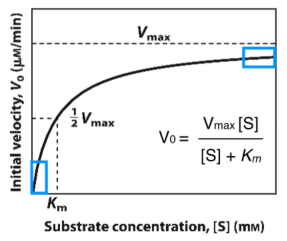
\includegraphics[width=0.45\textwidth]{MM}
	\caption{The blue box bottom left is when S << $K_{M}$, while the top right is when S >> $K_{M}$}
\end{figure}

Now, the actual derivation:

\begin{align*}
	&\text{E + S} \rightleftharpoons \text{ES} \xrightarrow{k_2} \text{E + P} \\[1ex]
	&\text{Rate of formation of [ES]} = k_1([E]_{\text{tot}} - [ES])[S] \\[1ex]
	&\text{Rate of breakdown of [ES]} = (k_{-1} + k_2)[ES] \\[1ex]
	&k_1([E]_{\text{tot}} - [ES])[S] = (k_{-1} + k_2)[ES] \\[1ex]
	&k_1[E]_{\text{tot}}[S] - k_1[ES][S] = (k_{-1} + k_2)[ES] \\[1ex]
	&k_1[E]_{\text{tot}}[S] = (k_1[S] + k_{-1} + k_2)[ES] \\[1ex]
	&[ES] = \frac{k_1[E]_{\text{tot}}[S]}{k_1[S] + k_{-1} + k_2} \\[1ex]
	&\text{Define } K_m = \frac{k_{-1} + k_2}{k_1} \Rightarrow [ES] = \frac{[E]_{\text{tot}}[S]}{[S] + K_m} \\[1ex]
	&V_0 = k_2[ES] = \frac{k_2[E]_{\text{tot}}[S]}{[S] + K_m} \\[1ex]
	&V_{\max} = k_2[E]_{\text{tot}} \Rightarrow V_0 = \frac{V_{\max}[S]}{[S] + K_m}
\end{align*}


\subsubsection{\gls{Lineweaver-Burk}}

Due to the asymptotic behavior of V0, it's difficult to determine $K_{M}$ and $V_{max}$ from it. Hence we create a double-reciprocal plot, which is linear, called the Lineweaver-Burk equation:


\begin{equation}
	\frac{1}{v} = \frac{K_m}{V_{\max}} \cdot \frac{1}{[S]} + \frac{1}{V_{\max}}
\end{equation}


where:
\begin{itemize}
	\item \( m = \frac{K_m}{V_{\max}} \) is the slope
	\item \( b = \frac{1}{V_{\max}} \) is the y-intercept
	\item \(c = -\dfrac{1}{K_{m}}\) is the x-intercept
\end{itemize}

\begin{figure}[h]
	\centering
	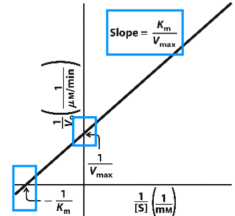
\includegraphics[width=0.45\textwidth]{LW-Burk}
	\caption{The blue boxes highlight the slope, y-intercept, and x-intercept of the Lineweaver-Burk equation. Those spots give are what make it so easy to find $K_{M}$ and $V_{max}$}
\end{figure}


\textbf{Derivation of the Lineweaver-Burk equation: }

We start with the Michaelis--Menten equation:

\begin{equation}
	v = \frac{V_{\max}[S]}{K_m + [S]}
\end{equation}

To linearize this, we take the reciprocal of both sides:

\begin{equation}
	\frac{1}{v} = \frac{1}{\frac{V_{\max}[S]}{K_m + [S]}}
\end{equation}

By inverting the fraction on the right-hand side:

\begin{equation}
	\frac{1}{v} = \frac{K_m + [S]}{V_{\max}[S]}
\end{equation}

Now split the numerator:

\begin{equation}
	\frac{1}{v} = \frac{K_m}{V_{\max}[S]} + \frac{[S]}{V_{\max}[S]}
\end{equation}

Which leaves us with the Lineweaver-Burk equation:

\begin{equation}
	\frac{1}{v} = \frac{K_m}{V_{\max}} \cdot \frac{1}{[S]} + \frac{1}{V_{\max}}
\end{equation}


\subsubsection{$K_{m}$ and $k_{cat}$}

The meaning of $K_{m}$ can vary greatly between different enzymes and even substrates.

One possible meaning for $K_{m}$ can be the following: if $k_{2}$ << $k_{-1}$ then $K_{m}$ essentially boils down to the following:
\begin{equation}
	K_{m} = \dfrac{k_{-1}}{k_{1}} = K_{D}
\end{equation}

So, for the case of $k_{2}$ << $k_{-1}$ $K_{m}$ tells us the affinity of a certain enzyme for its substrate. Note, that this is however only true in this one special case!

\textbf{$k_{cat}$ is the rate constant at the rate-limiting step}. This will often be $k_{2}$, however that is not always the case (especially if we have more than two reaction steps).

\subsubsection{Determining \gls{Enzyme Efficiency}}

The best way to determine the efficiency of an enzyme is by determining the following ratio:

\begin{equation}
	\frac{k_{\text{cat}}}{K_M}
\end{equation}

There is an upper limit to this ratio, set by the rate at which E and S can diffuse together. The \textbf{diffusion-controlled limit is $10^{8}$ to $10^{9} M^{-1}s^{-1}$}. Enzyme which have values close to this have achieved catalytic perfection.

PSA: this seems overkill from the lecture but there's a whole slide of it, so here is how we get the units by starting with the MM equation:

\begin{equation}
	v = \frac{k_{\text{cat}} [E]_T [S]}{K_m + [S]}
\end{equation}

When \( [S] \ll K_m \), the equation simplifies to:

\begin{equation}
	v \approx \frac{k_{\text{cat}}}{K_m} [E]_T [S]
\end{equation}

This resembles a second-order rate law: first order in both enzyme and substrate concentrations.

\bigskip

\textbf{Units:}
\begin{itemize}
	\item \( k_{\text{cat}} \): has units of \( \text{s}^{-1} \) (per second)
	\item \( K_m \): has units of \( \text{M} \) (molar, i.e., mol/L)
\end{itemize}

Thus, the specificity constant has units:

\begin{equation}
	\frac{k_{\text{cat}}}{K_m} = \frac{1\, \text{s}^{-1}}{1\, \text{M}} = \text{M}^{-1}\text{s}^{-1}
\end{equation}

\begin{figure}[h]
	\centering
	\subfigure[Km]{
		\includegraphics[width=0.45\textwidth]{KM}
	}
	\hfill
	% Second subfigure
	\subfigure[kcat]{
		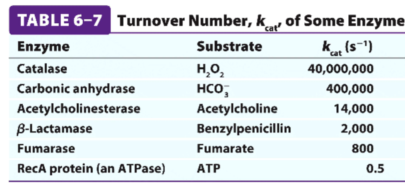
\includegraphics[width=0.5\textwidth]{kcat}
	}
		\subfigure[limit]{
		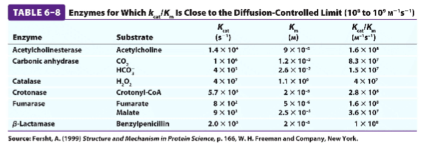
\includegraphics[width=0.5\textwidth]{limit}
	}
	\caption{Examples of rate for $K_{m}$, $k_{cat}$, and their ratio determining the enzyme's efficiency.}
\end{figure}

\subsubsection{$V_{max}$}

$V_{max}$ is the maximum initial velocity, and with that also the maximum velocity, that is attainable for a certain enzyme/substrate duo.

The equation for $V_{max}$ is the following:

\begin{equation}
	V_{\max} = k_{\text{cat}} \cdot [E]_T
\end{equation}

This equation comes from the fact we take the rate-limiting's step rate constant. Multiplying that with the enzyme concentration gives us the speed the enzymes can convert the substrate with at the choke point.

\subsection{\gls{Inhibition}}

Inhibitors are molecules that interfere with catalysis, decreasing or halting enzyme activity. They are critical for drug design, as nearly 50\% of all pharmaceutical agents are enzyme inhibitors. Inhibitors are classified into two main types:
\begin{itemize}
	\item Reversible Inhibitors: Interact transiently with the enzyme.
	\item Irreversible Inhibitors: Form a covalent bond or permanently alter the enzyme.
\end{itemize}

\subsubsection{\gls{Reversible Inhibition}}

Reversible inhibitors can act by competitive, non-competitive and uncompetitive mechanisms. The inhibition constant $K_{I}$ quantities the strength of inhibition in blocking the activity of an enzyme. To take this into account in kinetics, the factor $\alpha$ and $\alpha$' are used, where $\alpha$ is derived from $K_{I}$ (binding to enzyme) and $\alpha$' from $K^{'}_{I}$ (binding to enzyme-substrate complex).

\begin{figure}[h]
	\centering
	\includegraphics[width=0.45\textwidth]{Reversible_schematic}
	\caption{Types of Reversible Inhibition}
\end{figure}

\begin{itemize}
	\item \textbf{\gls{Competitive Inhibitor}}: The inhibitor competes with the substrate for the enzyme's active site. This increases $K_{m}$ but does not affect $V_{max}$.
	\item \textbf{\gls{Non-competitive Inhibitor}}: The inhibitor binds to a site other than the active site, reducing the concentration of the active enzyme-substrate complex. This decreases $V_{max}$, but does not affect $K_{m}$.
	\item\textbf{\gls{Uncompetitive Inhibitor}}: The inhibitor binds only to the enzyme-substrate complex, reducing the concentration of the active enzyme-substrate complex. Both $V_{max}$ and $K_{m}$ decrease.
\end{itemize}

\begin{figure}[h]
	\centering
	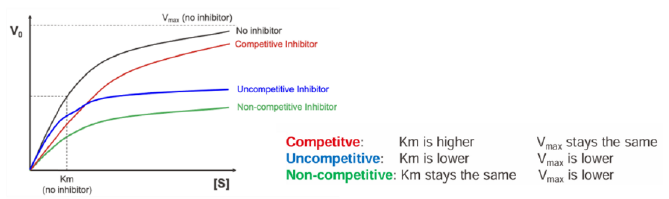
\includegraphics[width=0.45\textwidth]{reversible_MM}
	\caption{Impact of different Reversible Inhibition Types}
\end{figure}


\subsubsection{\gls{Irreversible Inhibition}}
Irreversible inhibitors form covalent bonds with the enzyme, \textbf{permanently inactivating} it.
Here are two types of irreversible inhibitors, their function, and usage:
\begin{itemize}
	\item \textbf{\gls{Suicide Inhibition}}: Also known as mechanism-based inactivators, these molecules are not reactive until they reach the active site, where they then go through the first steps of the reaction. At some point the inactivator becomes so reactive in a transition state it reacts irreversibly with the enzyme. Because these compounds are so highly specififc, and passive otherwise, they often have little side effects.
	\item \textbf{\gls{Transition-State Analogs}}: Molecules which are very similar to a transition-state. They bind significantly better to the enzyme and its active state than the substrate, making them an irreversible inhibitor.
\end{itemize}

\begin{figure}[h]
	\centering
	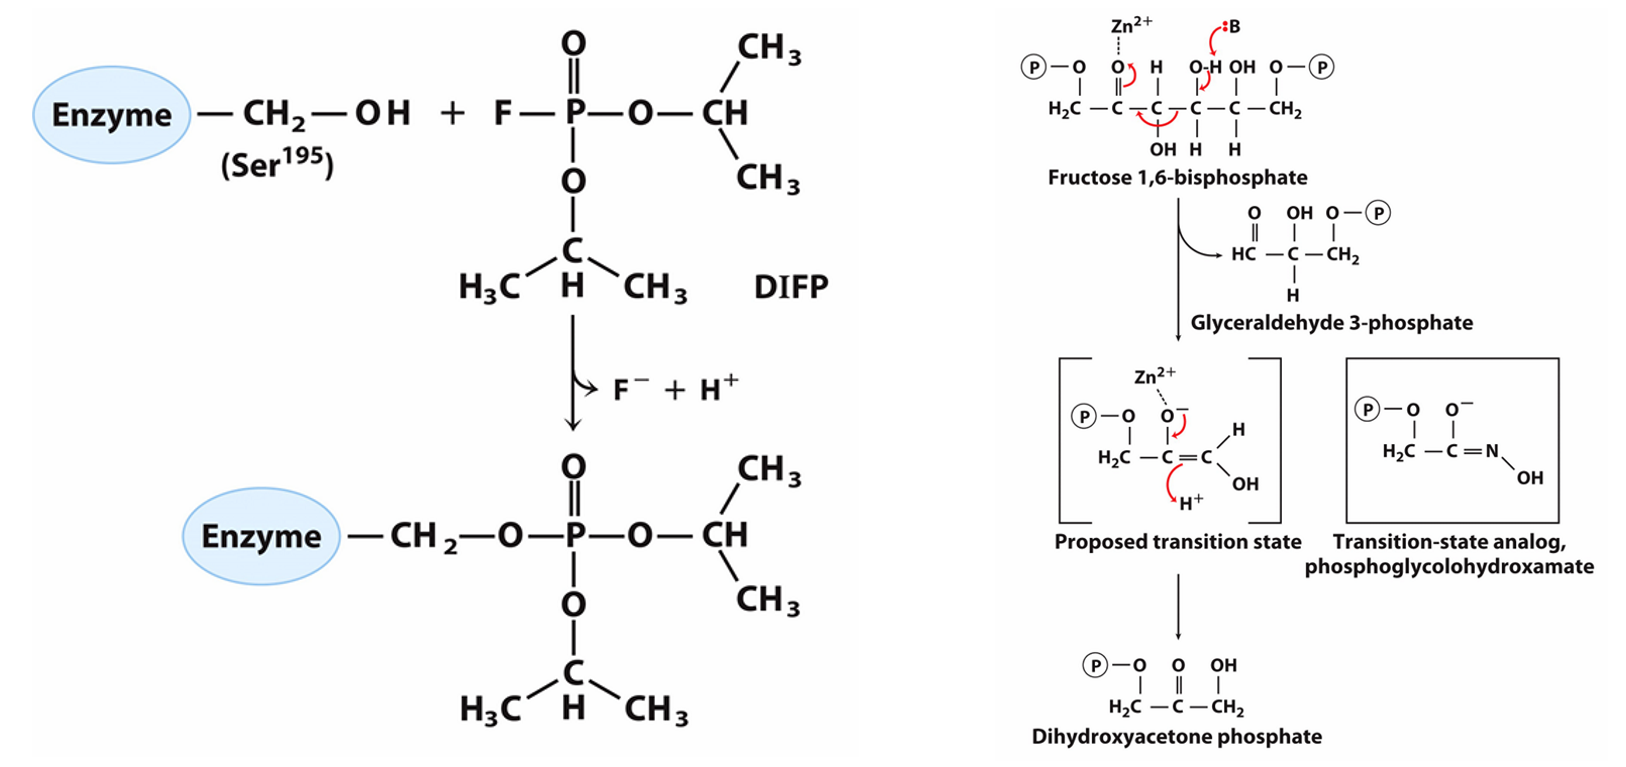
\includegraphics[width=0.45\textwidth]{Irreversible}
	\caption{Mechanism of different types of inhibition; on the left is a suicide mechanism and on the right a transition-state analog.}
\end{figure}



\end{document}